\documentclass[UTF8]{ctexart}
\usepackage{amsmath}
\usepackage{diagbox}
\usepackage{textcomp}
\usepackage{graphicx}
\usepackage{float}
\usepackage{caption}
\usepackage{adjustbox}
\usepackage{subfigure}
\usepackage{geometry}
\usepackage{pifont}
\usepackage{gensymb}
\usepackage{bm}
\usepackage{amstext}
\usepackage{amsfonts}
%引入代码块
\usepackage{listings}

\usepackage{xcolor}
%设置代码块格式

\definecolor{CPPGray}{RGB}{211,211,211}
\lstset{
 columns=fixed,       
 numbers=left,   % 在左侧显示行号
 numberstyle=\tiny\color{gray},% 设定行号格式
 frame=none,%none,% 不显示背景边框
 %aboveskip=1em,
 backgroundcolor=\color[RGB]{230,230,230},% 设定背景颜色
 keywordstyle=\color[RGB]{40,40,255},% 设定关键字颜色
 numberstyle=\footnotesize\color{darkgray},           
 commentstyle=\it\color[RGB]{0,96,96},% 设置代码注释的格式
 stringstyle=\rmfamily\slshape\color[RGB]{128,0,0},% 设置字符串格式
 showstringspaces=true,% 不显示字符串中的空格
 language=c++, % 设置语言
 morekeywords = {include,ull,int,double,return,static,typedef,if,else,for,long,void,class,struct,ll},                % 自加新的关键字(必须前后都是空格)
}

\begin{document}
\renewcommand{\thefootnote}{\fnsymbol{footnote}}
\newgeometry{left=2cm,bottom=3cm,right=2cm}
\linespread{1.4}
\title{\vspace{-5em}\heiti算法分析与设计基础\ \ 第五周作业\vspace{-2.5em}}
\date{}
\maketitle
\begin{center}
{\fangsong 徐浩博\quad 软件02\quad2020010108}
\end{center}


\subsection*{Problem 1}
首先我们用$\Theta(n)$的时间对每点计算$d_i=\sqrt{x_i^2+y_i^2}$,然后我们需要对$d_i$从小到大划出n个期望数量相等的区域,不如从圆的面积考虑,画出n个面积相等的圆环,设第i个圆环半径为$r_i$($0 \leq i\leq n$,特别地,$r_0=0$),则有
$$(r_i^2-r_{i-1}^2)=\pi/n$$
由此得:
$$r_i=\sqrt{\frac{i}{n}}$$
因此,我们对这n个点按照$d_i$放入n个桶中,使得放入第i号桶时有$\sqrt{\frac{i-1}{n}}\leq d_i\leq\sqrt{\frac{i}{n}}$,这一操作是$\Theta(n)$的,而且保证了一个点进入每个桶的概率都是$1/n$. 再运用桶排序,桶排序的时间复杂度也为$\Theta(n)$. 综合以上,我们得到了一个$\Theta(n)$的算法.


\subsection*{Problem 2}
我们的基本思路是对于a[1-n]的序列,取中间的那个k-QUANTILES,然后利用SELECT(书上已给出$\Theta(n)$复杂度的算法),以之为界将数组分治分为两半,分别递归求解. 考虑到如此递归的层数为$O(\log k)$,每层均为$\Theta(n)$,总复杂度为$O(n\log k)$.
\begin{lstlisting}[mathescape=true]
void PARTITION(int *A, int left, int right, int k, int gap)
{
	if(k <= 0 || left >= right)return;
	int mid_rank = (k + 1) / 2 * gap + left - 1;
	SELECT(A, left, right, mid_rank - left + 1);
	S.push_back(A[mid_rank]); #set S is what we want
	PARTITION(A, left, mid_rank, (k + 1) / 2 - 1, gap);
	PARTITION(A, mid_rank + 1, right, k - (k + 1) / 2, gap);
}
void GET_QUANTILES(int *A, int n, int k)
{
	int gap = n / k;
	if(n % k != 0) gap = gap + 1; #if n is not divisible by k
	PARTITION(A, 1, n, k - 1, gap);
}
\end{lstlisting}
严谨的复杂度求解如下:我们假设$k_0$为输入的k,那么
$$T(k) = 2T(k/2) + O(nk/k_0)$$
因此
\begin{align*}
	T(k_0)&= 2T(\frac{k_0}{2}) + O(n)\\
	&=2[T(\frac{k_0}{4})+O(\frac{nk_0}{2\times k_0})]+O(n)\\
&=2T(k/4)+2O(\frac{n}{2})+O(n)\\
&=\cdots\\
&=\overbrace{O(n)+\cdots+O(n)}^{\log_2k\textbf{个}}\\
&=O(n\log k)
\end{align*}

\newpage
\section*{各种排序算法时间开销比较实验报告}
\subsubsection*{摘要}
{\kaishu\normalsize  斐波那契数列可谓是世界上最为著名的数列之一,虽然可以通过数学方法找到通项公式,但在实际通过程序运算时,仍可能存在诸多问题. 本文介绍了编程计算斐波那契数的四种常见算法,并通过编写C++程序,对比各种算法的性能,包括计算结果误差和时间开销等. 通过对比,我们认为通项公式法实际上是一种编程上不太可行的算法,而通过矩阵乘法实现的logn复杂度的算法可以作为实际计算斐波那契数的一种理想的方法.}
\subsubsection*{关键词:插入排序\ \ 希尔排序\ \ 快速排序\ \ 归并排序\ \ 基数排序\vspace{1.5em}}

\section*{1\ \ \ 实验环境}
操作系统:Windows 10\par
IDE:Visual Studio 2019\par
处理器:Intel Core i7-10750H 六核CPU @ 2.60GHz\par
编程语言:C++11

\section*{2\ \ \ 算法分析}
\subsection*{2.1\ 插入排序}
插入排序是每一轮依次将数组后方的数字插入前面已排好的数字之中. 考虑到n个数,每个数a[i]都需要对前面i个已排好的数进行向前插入,因此复杂度为$O(n^2)$.
\subsection*{2.2\ 希尔排序}
希尔排序是把记录按下标的一定增量分组,对每组使用插入排序算法排序;随着增量逐渐减少,每组包含的关键词越来越多,当增量减至1时,整个数组恰被分成一组,算法便终止. 该种方法时间复杂度一般小于$O(n^2)$又大于$O(n)$,在精心挑选的减少量下,它的均摊复杂度可以达到$O^(n^1.17)$. 本实验中,我们简单地将gap从n/2开始每次减半,并认为它的复杂度为$O(n^{1+r})$,其中r是一个不大于1的正数.
\subsection*{2.3\ 快速排序}
课本上改进过的快速排序需要随机选择一个序列中的数作为pivot,而考虑到本实验中数据为随机生成的,且C++的rand在数据规模大时时间开销十分可观,因此我们直接采用最右边的元素作为pivot. 课堂上已分析过,本算法均摊复杂度为$O(nlogn)$.
\subsection*{2.4\ 归并排序}
归并排序是每次将数组划分为两半利用递归分别排序,之后合并在一起,是一种分治算法. 课堂上也分析过,本算法均摊复杂度为$\Theta(nlogn)$.

\subsection*{2.5\ 基数排序}
课堂上已分析过,基数排序对于给定b位数和正整数r,总时间为$\Theta((b/r)(n+2^r))$,本实验中,我们取$r=log(n),\ b=\log_{r}{MAXNUM}=O(logn)$,因此算法复杂度为$\Theta(n)$,是线性的.


\section*{3\ \ \ 实验设计思路}
考虑到插入排序为$O(n^2)$复杂度的算法,运算较慢,因此进行排序的数据规模不宜过大. 因此,我们对插入排序进行数据规模$n=10, 10^2, 10^3, 10^4, 10^5, 10^6$的实验并计时;对于希尔排序、快速排序、归并排序、基数排序,我们分别对$n=10, 10^2, 10^3, 10^4, 10^5, 10^6, 10^7, 10^8, 2\times 10^8$进行验证. 与此同时,当数据规模小于等于$10^6$时,我们采用测量5次并平均的方法减少实验误差.

\section*{4\ \ \ 结果分析}
首先,我们多次对照了规模较小$n=100$时五种排序的排序结果,结果均一致,表明我们的排序算法是正确的. 然后,我们将按照实验设计思路,对不同n下的实际运行时间. 我们将运行结果以表格的形式列出. 
\begin{table}[H]
	\begin{center}
    \centering{\caption{不同排序算法在不同数据规模下的时间开销表(单位:微秒)}}
		\begin{tabular}{c|c|c|c|c|c}
			\hline
			n&插入排序&希尔排序&快速排序&归并排序&基数排序\\
			\hline
			\hline
			10 &9.2&	6.7	&7.5&	8.1	&45.3\\
			\hline
			$10^2$ & 52.1	&17.4	&22.8	&14.5	&38.3\\
			\hline
			$10^3$ & 3913.9	&189	&275.4&	149.4&	201\\
			\hline
			$10^4$ & 3.40639$\times{10^5}$	&2984.5	&1961.7&	1359.1&	2024.2\\
			\hline
			$10^5$ & 3.25148$\times{10^7}$&	53866.7	&23642.9&	15034.8&	14220.2\\
			\hline
			$10^6$ &N/A& 8.40005$\times{10^7}$	&3.00016$\times{10^5}$	&1.95037$\times{10^5}$&	1.51394$\times{10^5}$\\
			\hline
			$10^7$ &N/A& 1.37058$\times{10^7}$&	3.322940$\times{10^6}$	&2.110910$\times{10^6}$&	1.439760$\times{10^6}$\\
			\hline
			$10^8$ &N/A& 2.32647$\times{10^8}$	&3.74192$\times{10^7}$	&2.3976$\times{10^7}$&	1.45465$\times{10^7}$\\
			\hline
			$2\times 10^8$&N/A & 5.66246$\times{10^8}$&	7.66161$\times{10^7}$	&4.88346$\times{10^7}$	&2.86977$\times{10^7}$\\
			\hline
		\end{tabular}
\end{center}\end{table}
我们将$n=10-10^5$时5种排序方法的时间开销绘制成图:
\begin{figure}[H]\begin{center}
	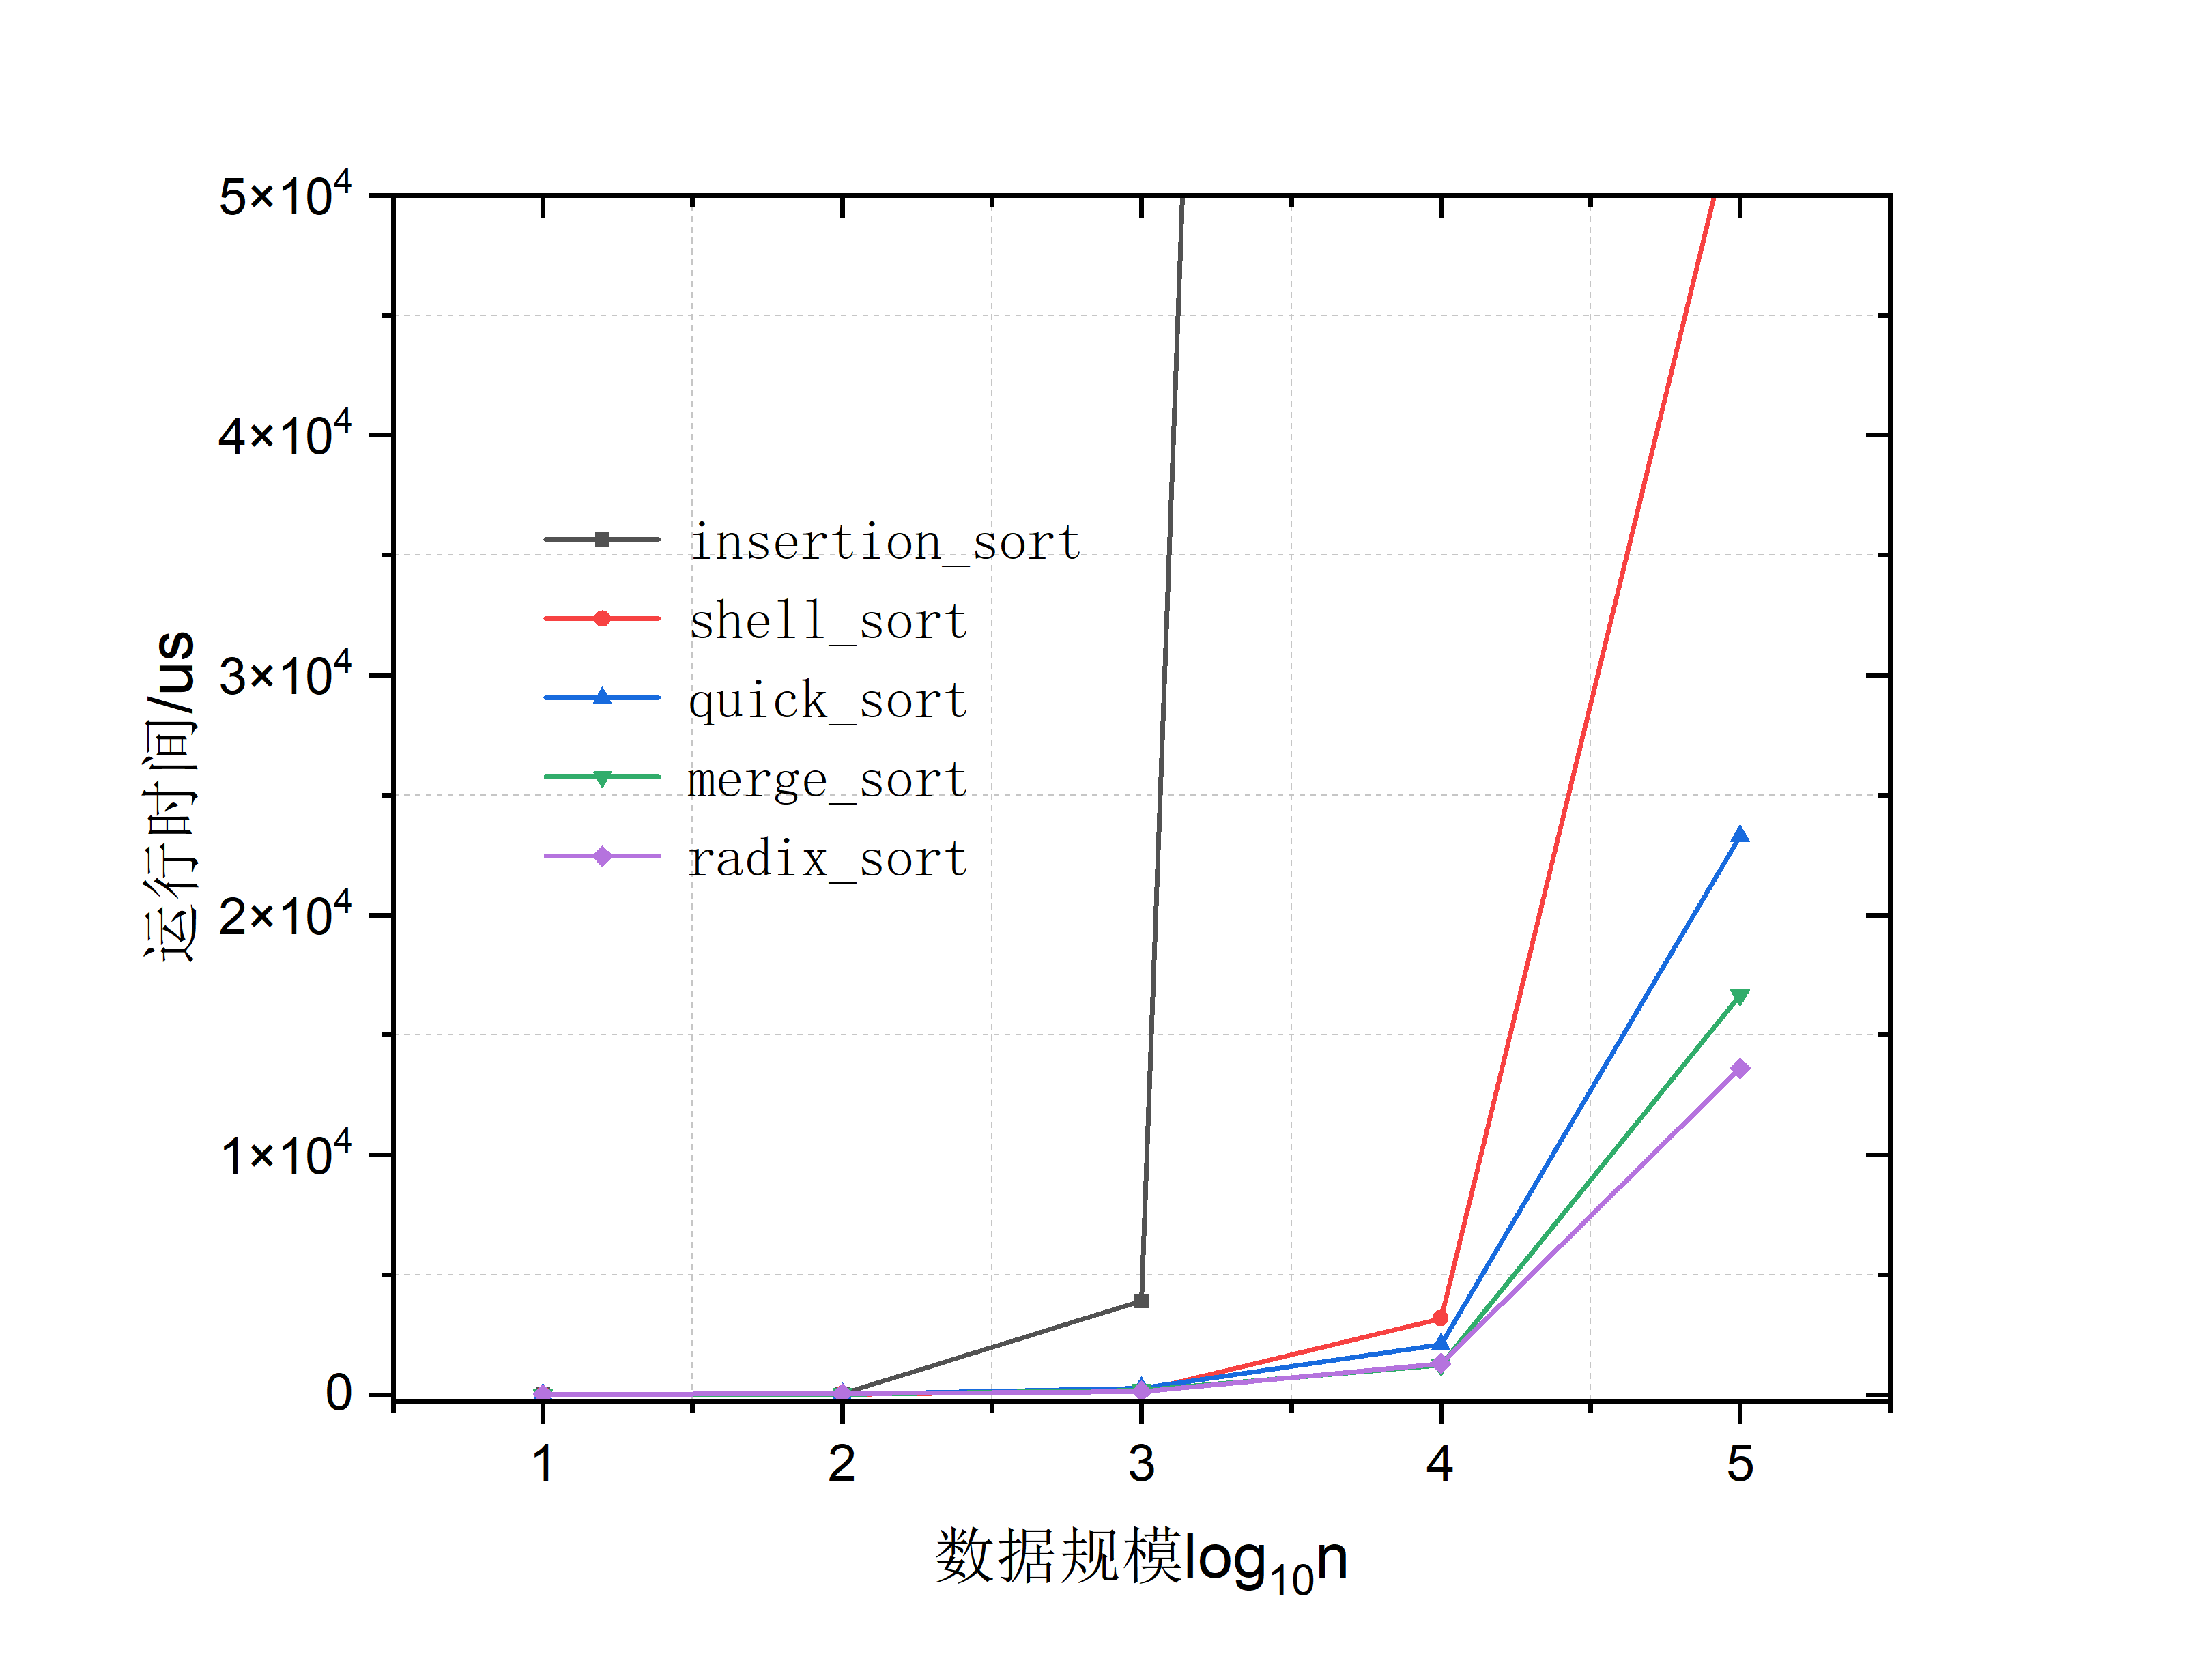
\includegraphics[scale=0.5]{graph1.png}
\caption{小规模数据运算时间对比图($n\in [10,\ 10^5]$)}
\end{center}\end{figure}
可以很明显看出,数据规模较小$n\leq 100$时,五种方法运算事件几乎一样;而数据规模稍大($n\geq 1000$)时,$O(n^2)$的插入排序明显慢于剩余四种排序. 我们也可以清楚看到,$n=10^5$时,希尔排序也显著慢于其余几种排序,我们再将n调大,看看剩余四种排序的情况:
\begin{figure}[H]\begin{center}
	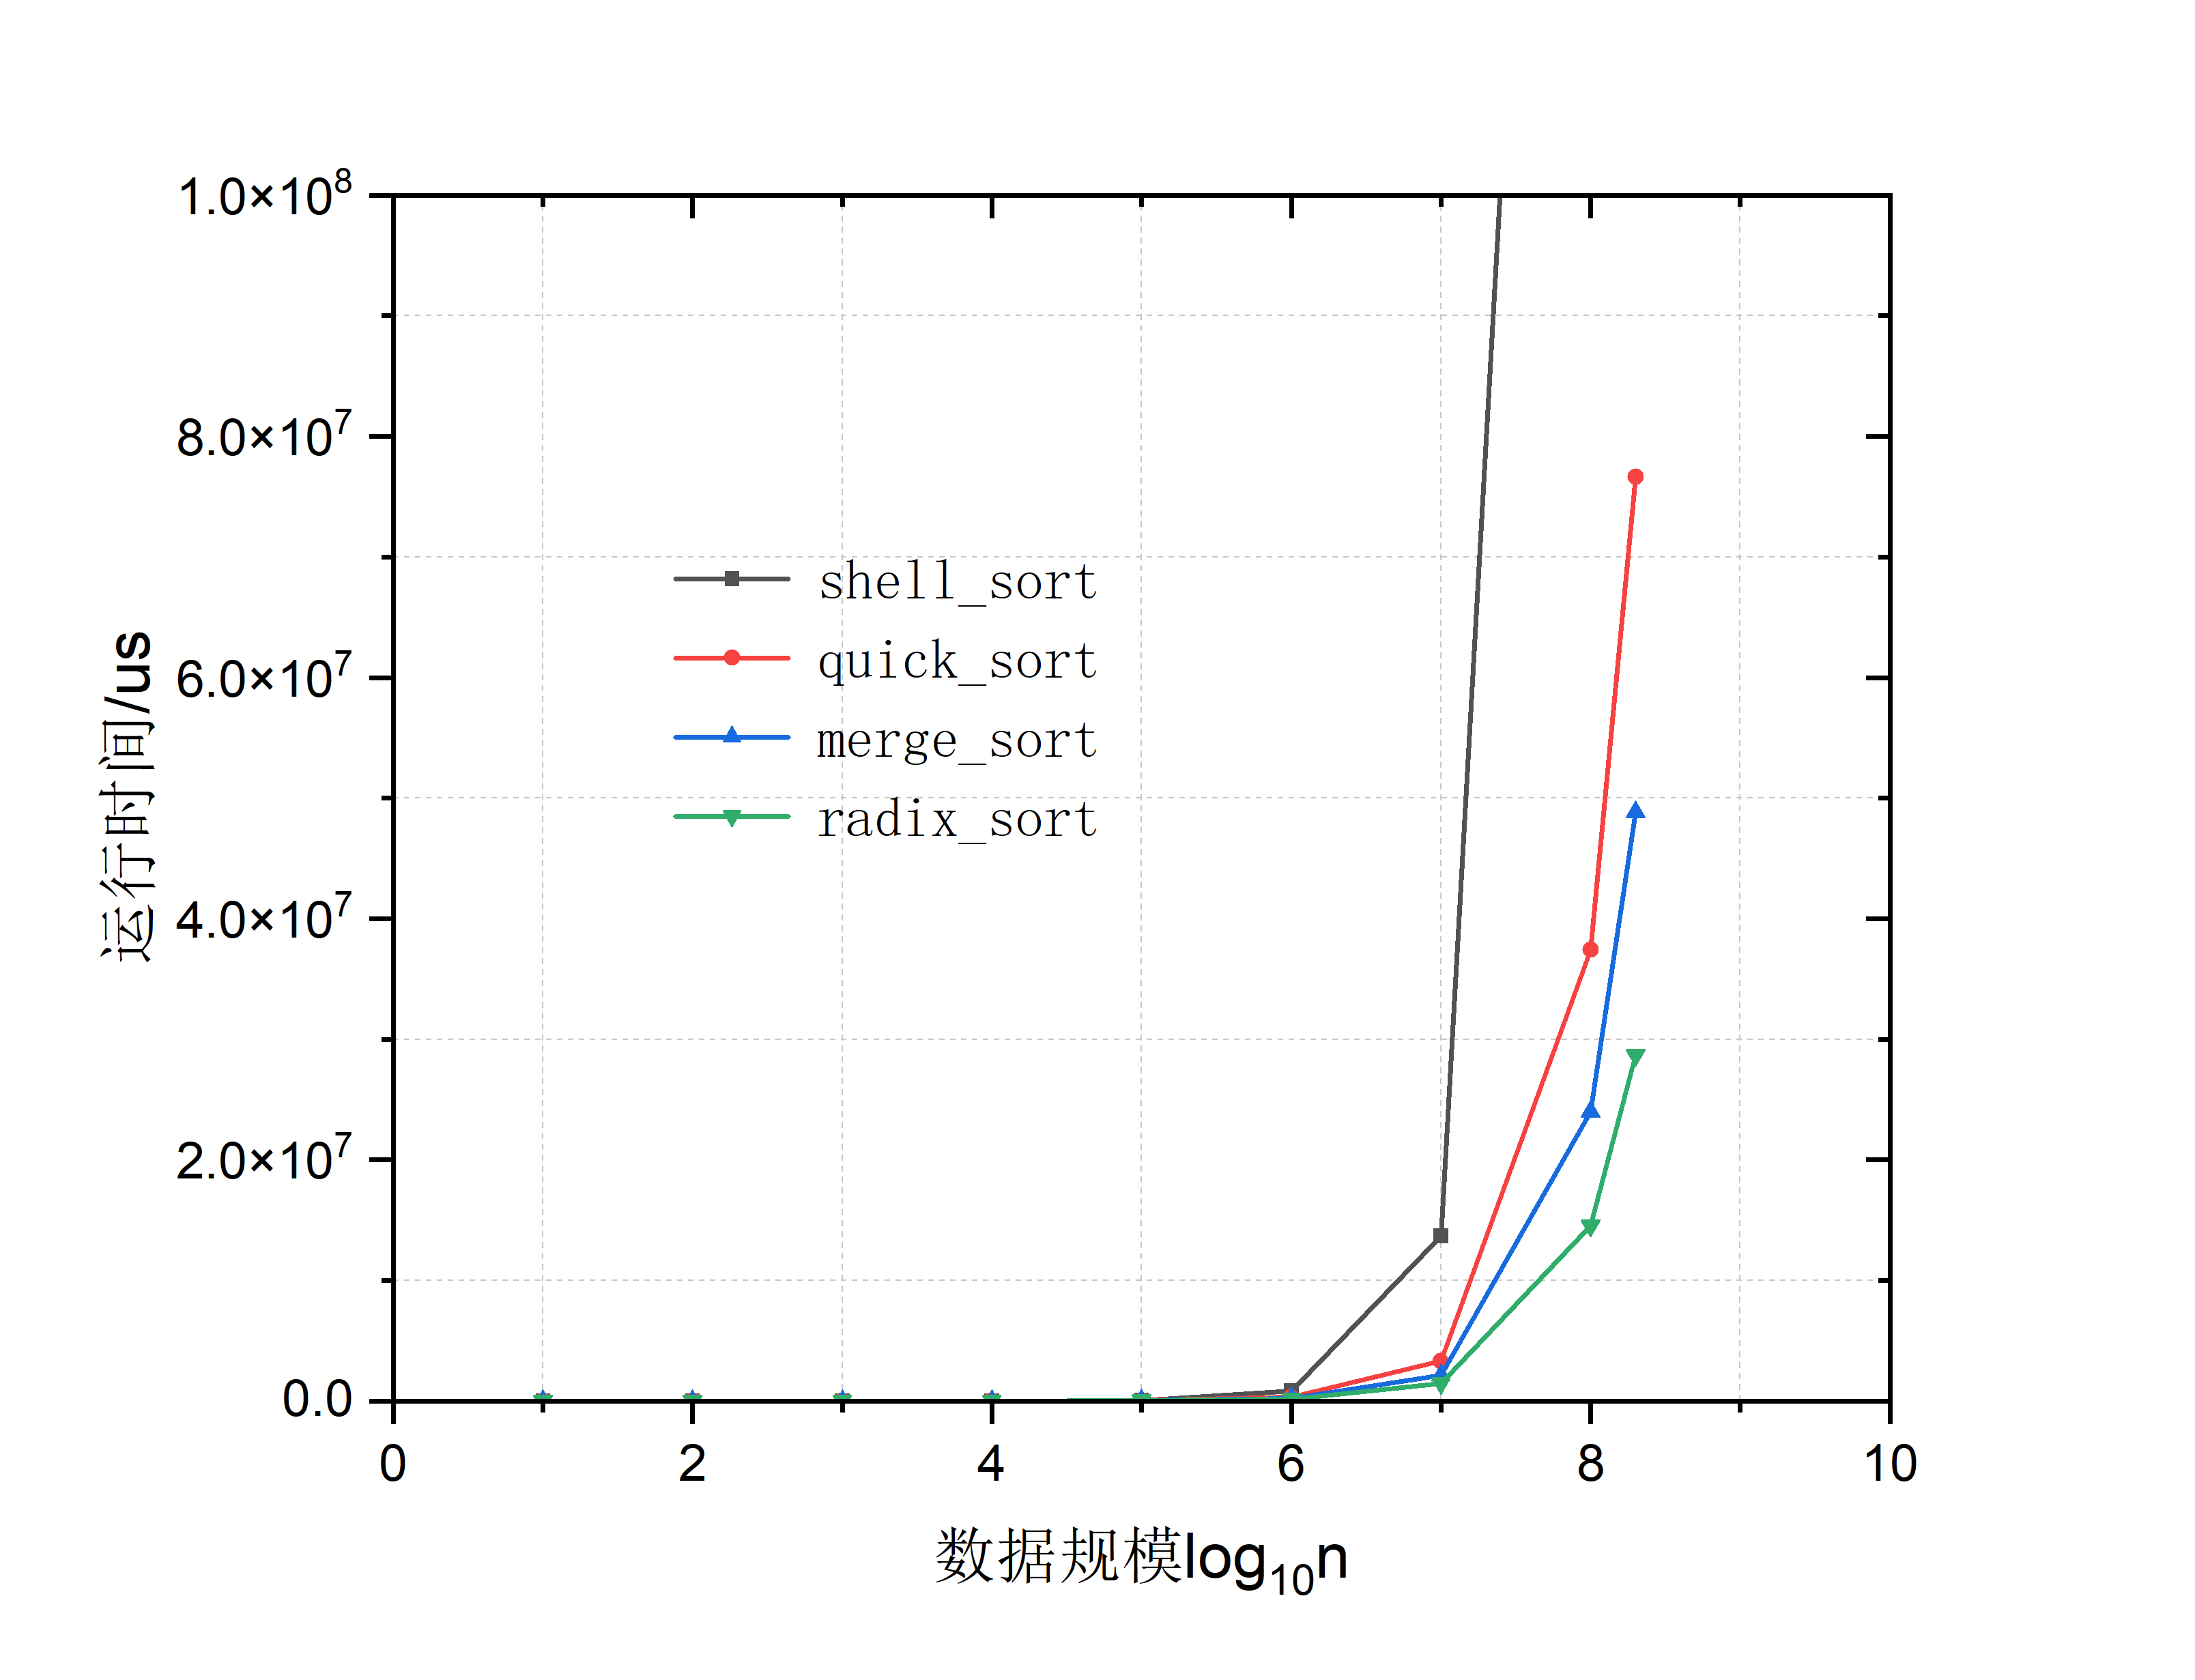
\includegraphics[scale=0.5]{graph2.png}
\caption{大规模数据运算时间对比图($n\in [10,\ 2\times 10^8]$)}
\end{center}\end{figure}
可以看到,$O(n^{1+r})$的希尔排序显著慢于其余几种O(nlogn)或线性的排序算法. 其次我们看到,同为O(nlogn)的快速排序略慢于归并排序;它们又都慢于线性的基数排序.


\section*{4\ \ \ 总结}
可以看到,平方复杂度的插入排序果然是五种算法中最慢的一种排序算法,而希尔排序也较慢于剩下几种nlogn或线性复杂度的算法. 在nlogn算法中,快速排序略慢于归并排序,它们又都略慢于基数排序,但三者运行速度基本在同一个量级. 事实上,由于算法复杂度的常数不定,计算机环境不同,这三种排序算法的快慢是很难通过理论得到的,实践证明了“快速”的快速排序反而不是最快的;但考虑到基数排序和归并排序需要额外的辅助空间,而当n足够大时,辅助空间就显得格外累赘,可能会影响到主存的使用. 因此大多数情况下,快速排序是一个不坏的选择.

\end{document}
